%%%%%%%%%%%%%%%%%%%%%%%%%%%%%%%%%%%%%%%%%
% University/School Laboratory Report
% LaTeX Template
% Version 3.1 (25/3/14)
%
% This template has been downloaded from:
% http://www.LaTeXTemplates.com
%
% Original author:
% Linux and Unix Users Group at Virginia Tech Wiki 
% (https://vtluug.org/wiki/Example_LaTeX_chem_lab_report)
%
% License:
% CC BY-NC-SA 3.0 (http://creativecommons.org/licenses/by-nc-sa/3.0/)
%
%%%%%%%%%%%%%%%%%%%%%%%%%%%%%%%%%%%%%%%%%

%----------------------------------------------------------------------------------------
%	PACKAGES AND DOCUMENT CONFIGURATIONS
%----------------------------------------------------------------------------------------

%\documentclass{article}
\documentclass[10pt]{sig-alternate-05-2015}
\usepackage{graphicx}
\usepackage{subfigure,epsfig,float}
\usepackage{epstopdf}
\usepackage{color}
\usepackage{enumitem}

\usepackage[version=3]{mhchem} % Package for chemical equation typesetting
\usepackage{siunitx} % Provides the \SI{}{} and \si{} command for typesetting SI units
\usepackage{graphicx} % Required for the inclusion of images
\usepackage{natbib} % Required to change bibliography style to APA
\usepackage{amsmath} % Required for some math elements 
\usepackage{url}
\setlength\parindent{0pt} % Removes all indentation from paragraphs

\renewcommand{\labelenumi}{\alph{enumi}.} % Make numbering in the enumerate environment by letter rather than number (e.g. section 6)

%\usepackage{times} % Uncomment to use the Times New Roman font

%----------------------------------------------------------------------------------------
%	DOCUMENT INFORMATION
%----------------------------------------------------------------------------------------

\title{Fibonacci Heap \\ \textsc{University of Colorado Boulder} \\ \textsc{CSCI 5454 - Design and Analysis of Algorithms} \\ \textsc{2016} } % Title

\author{Mahesh Kumar Ravindranathan } % Author name

\date{\today} % Date for the report

\begin{document}


\maketitle % Insert the title, author and date


\section{Introduction to Fibonacci Heap}
Fibonacci Heap is a data structure that is generally used for priority queue operations, consisting of a collection of heap-ordered trees~\cite{wikiFiboHeap,cormen2009introduction} . The data structure was developed by Micheal L.Fredman and Robert E. Tarjan in 1984. They are named Fibonacci Heaps because their running time analysis is based on Fibonacci numbers. \\

Fibonacci heap is a collection of min-heap-ordered trees (The data contained in each node is less than or equal to the data  in the node's children). In Fibonacci heaps, the trees are rooted but unordered. Each node contains a pointer to its parent and a pointer to any one of its children. The children are linked together in a circular, doubly linked list. The order in which the siblings appear in a child list is arbitrary. The number of children in the child list of a node is stored as degree. Boolean value is used to mark a node which indicates whether  the node has lost a child since the last time it was made the child of another node.\\

\begin{figure}
	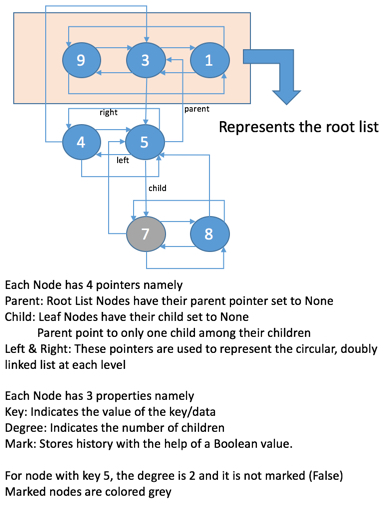
\includegraphics[width=0.95\columnwidth]{Figures/FibonacciHeap}
	\caption{Fibonacci Heap Example}
\end{figure}

For simplicity, the future figures won't have the representation of the doubly linked list left and right pointer. I will be representing just the parent pointer. The orange layer indicates the root list.



\section{Operations of Fibonacci Heap}
The various operations of the Fibonacci Heaps are as follows:
\begin{itemize}
	\item Inserting a node
	\item Union of Fibonacci Heaps
	\item Extracting the Minimum Node
	\item Decreasing a key
	\item Deleting a node
\end{itemize}

Let us consider $n$ to be the number of nodes in the Fibonacci Heap.

\subsection{Inserting a node}
In Fibonacci Heap, inserting a node is $O(1)$ operation since it is equivalent to adding a node to a circular, doubly linked list called the root list. The added node has no children and is unmarked.

\subsection{Union of Fibonacci Heaps}
In Union operation, the root list of both the Fibonacci Heaps are united  and the new minimum node is determined. The amortized cost of the union operation is $O(1)$ as well.

\subsection{Extracting the Minimum Node}
In the process of extracting the minimum node, the minimum node is extracted from the Fibonacci Heap. The procedure followed is as follows:
\begin{itemize}
	\item The minimum node's children are added to the root list.
	\item Consolidate the root list by linking roots when they are of equal degree.
	\item Repeat the previous step until at most one root remains of each degree.
\end{itemize}
The amortized cost of extracting a minimum node is $O(\lg{n})$

\subsection{Decreasing a key}
In this process, we decrease the value of the key for an existing node. If the min-heap order is not violated, no changes are required. If the min-heap order is violated, many changes can occur. The procedure followed is as follows:
\begin{itemize}
	\item We cut the node from it's parent.
	\item Add the node to the root list.
	\begin{itemize}
	\item If the parent is not marked: No action taken.
	\item If the parent was already marked, it would be added to the root list as well and this step occurs recursively up the tree until either a root or an unmarked node is found.
	\end{itemize}
\end{itemize}
The amortized cost of decreasing a key is $O(1)$

\subsection{Deleting a node}
Deleting a node is equivalent to decreasing a key and then extracting the minimum node for a Fibonacci Heap and hence it has an amortized cost of $O(\lg{n})$
\section{Fibonacci Heap Implementation}

For the implementation of the Fibonacci Heap, I created a FibonacciHeap class and a Node class.
The FibonacciHeap Node class has the following variables:
\begin{itemize}
	\item key: Indicates the value of the key(data)
	\item degree: The number of immediate child nodes
	\item parent: The parent of the node
	\item child: The child of the node
	\item left \& right: The siblings if any are pointed using these pointers (circular, doubly linked list)
	\item mark: Used for tracking history and restricting the amortized cost for extracting minimum and deleting a node to $O(\lg{n})$  
\end{itemize}
The FibonaaciHeap class has the following variables: 
\begin{itemize}
	\item rootList: Pointer to a node of the root list
	\item minNode: Node with the minimum key value
	\item totalNode: Total number of nodes within the Fibonacci Heap
\end{itemize}
The FibonacciHeap class has multiple functions defined, their uses are as follows:
\subsection{ insert (Insert a node to the Fibonacci Heap) }
\begin{itemize}
		\item We create a new node
		\item Make left and right pointer point to itself
		\item Call the mergeNewNodeWithRootList function
		\item If minNode was undefined or it has key greater than the new node, we update minNode to point to the new node
		\item We increase the totalNode count by 1 indicating that a new node was added to the Fibonacci Heap.
\end{itemize}

\subsection{ extractMin ( Extracting the Minimum Node ) }
	\begin{itemize}
		\item We check if the minNode is undefined or not
		\item If minNode does exist, we check if the node has child node
			\begin{itemize}
			\item If there exist a child Node, then we get the list of all the children using the iterateNodeDoubleLinkList function
			\item We add all the children to the root list using the mergeNewNodeWithRootList function
			\end{itemize}
		\item We remove the minimum node from the root list using the removeFromRootList function
		\item We update the minNode to a random node in the root list
		\item We call the consolidate function 
		\item We decrease the total nodes by 1 as the minimum node is removed from the Fibonacci Heap
	\end{itemize}
	
\subsection{consolidate ( Reduce the number of min-heap trees from the Fibonacci Heap )}
		\begin{itemize}
			\item We create an empty list of size ( total number of nodes in the Fibonacci Heap ) called A
			\item We get all the nodes in the root list using the  iterateNodeDoubleLinkList function
			\item For each node, we iterate and get it's degree
			\begin{itemize}
				\item If the list A, has any node corresponding to the degree
				\item We figure out which node has lower key value and add the larger key value node as a child to the lower key value node using the heapLink function
				\item We update the list A with index as degree of the node to empty
				\item We increment the degree of the node by 1
			\end{itemize}
			\item We update the minNode with the node which is minimum among the root list
		\end{itemize}
\subsection{decreaseKey ( Decreasing a key and updating the Fibonacci Heap)}
		\begin{itemize}
			\item If the min-heap property is violated
			\begin{itemize}
				\item We run the cut function
				\item We run the cascadingCut function
			\end{itemize}
			\item We update the minNode appropriately.
		\end{itemize}
\subsection{ cut ( If the child node is smaller than its parent after the decrease key operation, we cut the child and bring it back to the root list )}
		\begin{itemize}
			\item We call the removeFromChildList function
			\item We decrease the degree by 1 and call the mergeNewNodeWithRootList function to add the removed child to the root list
			\item We mark the parent to empty and unmark it when it is added to the root list
		\end{itemize}
\subsection{ cascadingCut ( Based on the history ( mark property ), we decide if we need to recursively go up the tree, post a cut operation )}
		\begin{itemize}
			\item If the node is not marked, we mark it
			\item If the node has been marked already, we recursively iterate up to the root or until a node is not marked by calling the cut and cascadingCut function.	
		\end{itemize}
\subsection{heapLink ( Remove a node from the rootList and add it as a child to another node of the rootList, maintaining the circular double linked list properties)}
		\begin{itemize}
			\item Call the removeFromRootList function for the node that needs to be removed from the root list.
			\item Call the mergeWithChild function to merge the node as a child of another node
			\item Increase the degree of the node to which the node is added as child, update hat parent pointer and update the mark to False
		\end{itemize}
\subsection{removeFromRootList ( Remove a node from the circular double linked root list )}
		\begin{itemize}
			\item If the pointer rootList is pointing to it, update the pointer to another node in the root list
			\item Update the pointer of the doubly linked list to remove the node
		\end{itemize}
\subsection{iterateNodeDoubleLinkList ( Iterating through the circular double linked list for a given node )}
		\begin{itemize}
			\item If the node is undefined, return none.
			\item If the node is defined, iterate through a particular direction of the doubly linked list till we reach back to the original node. 
			\item Return all the nodes that were traversed through.
		\end{itemize}
\subsection{mergeRootListWithExistingRootList ( Joining two circular doubly linked root list )}
		\begin{itemize}
			\item Update the pointers to join both the doubly linked lists of root list
		\end{itemize}
\subsection{mergeNewNodeWithRootList ( Adding a node to doubly linked root list )}
		\begin{itemize}
			\item If the rootList pointer is empty update the pointer to point to the node
			\item If the rootList pointer is not empty, add the node to the circular doubly linked root list
		\end{itemize}
\subsection{mergeWithChild ( Adding a node as the child of a given parent node )}
		\begin{itemize}
			\item If the parent has no child, just update the child pointer to point to the node
			\item If the parent has a child already, update the pointers to add the node to circular doubly linked list that contains all its children.
		\end{itemize}
\subsection{removeFromChildList ( Removing a node from its parent )}
		\begin{itemize}
			\item If it is the only child, update the parent's child pointer as empty
			\item If the parent had multiple child, update parent pointer with another child and the child's parent pointer with the parent node
			\item Update the pointers to remove the node from the circular doubly linked list
		\end{itemize}


\section{Mathematical Analysis}
We use potential method to analyze the performance of Fibonacci Heap Operations. For a Fibonacci Heap H, let us indicate the number of trees in the root list of H by $t(H)$ and the number of marked nodes in H by $m(H)$. \\ The potential of Fibonacci Heap H is defined by \\
\begin{center}
	$\Phi{H} \ = \ t(H) + 2m(H)$
\end{center}
Clearly,
\begin{itemize}
	\item The potential when there is no heaps is zero.
	\item The potential is non-negative at all subsequent times.
	\item The amortized cost upper bounds the actual cost
\end{itemize}

The Mathematical Analysis for the run time of the various operations are as follows:

\subsection{Inserting a node}
Initial potential:
\begin{center}
	$\Phi{(H)} \ = \ t(H) + 2m(H)$
\end{center}
After insertion of a node, let the Fibonacci heap be denoted by $H'$.
\begin{center}
$t(H') \ = \ t(H) + 1$ \\
$m(H') \ = \ m(H)$ \\
\end{center}
Increase in potential = New potential - Old potential
\begin{equation}
	\begin{split}
		\triangle{\Phi} &= [t(H')+2m(H')] - [t(H)+2m(H)]
		\\&= [t(H) + 1 + 2m(H)] - [t(H)+2m(H)]
		\\&= 1
	\end{split}
\end{equation}
Amortized cost = Actual cost + Increased potential
\begin{equation}
\begin{split}
Amortized \ cost &= O(1) + 1
\\&= O(1)
\end{split}
\end{equation}
\subsection{Union of Fibonacci Heaps}
Initial potential:
\begin{center}
	$\Phi{(H_1)} \ = \ t(H_1) + 2m(H_1)$ \\
	$\Phi{(H_2)} \ = \ t(H_2) + 2m(H_2)$
\end{center}
Let Fibonacci Heap tree formed by the union of $H_1$ and $H_2$ be denoted by $H'$
\begin{center}
$t(H') \ = \ t(H_1) + t(H_2)$ \\
$m(H') \ = \ m(H_1) + m(H_2)$ \\
$\Phi{(H')} \ = \ t(H') + 2m(H')$
\end{center}
Increase in potential is given by
\begin{equation}
	\begin{split}
		\triangle{\Phi} &= [t(H')+2m(H')] \\ 
		& - [ (t(H_1) + 2m(H_1)) + (t(H_2) + 2m(H_2)) ]
		\\&= [ (t(H_1) + 2m(H_1)) + (t(H_2) + 2m(H_2)) ] \\
		& - [ (t(H_1) + 2m(H_1)) + (t(H_2) + 2m(H_2)) ]
		\\&= 0
	\end{split}
\end{equation}
Amortized cost = Actual cost + Increased potential
\begin{equation}
\begin{split}
Amortized \ cost &= O(1) + 0
\\&= O(1)
\end{split}
\end{equation}
\subsection{Extracting the Minimum Node}
Initial potential:
\begin{center}
	$\Phi{(H)} \ = \ t(H) + 2m(H)$
\end{center}
The actual cost of extracting the minimum node can be accounted as follows: 
\begin{itemize}
	\item An $O(D(n))$ contribution comes from there being at most $D(n)$ children of the minimum node that are added to the root list and processed.\\
	\item The size of the root list on calling the consolidate function is at most $D(n)+t(H)-1$, since there were originally $t(H)$ trees, at most $D(n)$ of nodes can be the children to the node that is being extracted and one $(1)$ since that is the node that is being extracted. Thus the total actual work done in extracting the minimum node is $O(D(n)+t(H))$
\end{itemize}
The change in potential is given as follows:
\begin{itemize}
	\item Potential at most, post extracting the node is \\ $(D(n)+1 + 2m(H))$, since at most $D(n)+1$ roots remain and no nodes become marked during the operation.
\end{itemize}
Amortized cost = Actual cost + Increased potential
\begin{equation}
\begin{split}
Amortized \ cost &= O(D(n)+t(H)) \\
& + [ [(D(n)+1+2m(H)] - [t(H)+2m(H)] ]
\\&= O(D(n)) + O(t(H)) + D(n) + 1 -t(H)
\\&= O(D(n))
\end{split}
\end{equation}
\subsection{Decreasing a key}
Initial potential:
\begin{center}
	$\Phi{(H)} \ = \ t(H) + 2m(H)$
\end{center}
The actual cost for decreasing a key can be accounted as follows: 
\begin{itemize}
	\item It takes $O(1)$ time, plus the time to perform cascading cuts.
	\item Suppose the cascading cut is recursively called $c$ times and each call takes $O(1)$ time exclusive of recursive call, it takes $O(c)$ including all recursive call.
\end{itemize}
The change in potential is given as follows:
\begin{itemize}
	\item Each recursive call of cascading cut, except for the last one, cuts a marked node and clears the marked bit.
	\item There are hence, $(t(H) + c)$ trees
	\item There are at most $( m(H) - c + 2 )$ marked nodes
\end{itemize}
Amortized cost = Actual cost + Increased potential
\begin{equation}
	\begin{split}
		Amortized \ cost &= O(c) \\
		& + [ (t(H) + c) + 2(m(H) - c + 2) - [t(H)+2m(H)] ]
		\\&= O(c) - c + 4
		\\&= O(1)
	\end{split}
\end{equation}
\subsection{Deleting a node}
Deleting a node is equivalent to decreasing a key and then extracting the minimum.\\
Hence, 
\begin{equation}
	\begin{split}
		Amortized \ cost &= O(D(n)) + O(1)\\
		\\&= O(D(n))
	\end{split}
\end{equation}
\subsection{Bounding the maximum degree}
To show that the Extracting the minimum node operation and the Deleting a node operation takes $O(\lg{n})$ we need to prove that the upper bound of $D(n)$ on the degree of any node of a $n$-node Fibonacci heap is $O(\lg{n})$. \\ \\
Let x be any node in a Fibonacci Heap, and suppose the $degree[x] = k $. If $y_1, y_2, y_3,...,y_k$ denote the children of $x$ in the order in which they were linked to $x$, from the earliest to the latest. Then, $degree[y_1] \geq \ 0$ and $degree[y_i] \geq \ i - 2$ for $i=2,3,...,k$ because when $y_i$ was linked to $x$, all of $y_1,y_2,...,y_{i-1}$ were children of $x$, so we must have had $degree[x] \geq \ i-1$. Node $y_i$ is linked to $x_i$ only if their degree are the same and hence $degree[y_i] = degree[x] \geq i - 1$. Since then, $y_i$ has lost at most one child, since it would have been cut from x if it had lost two children. We conclude that $degree[y_i] \geq i-2$\\ \\
From the property of Fibonacci number: We have
\begin{center}
	$F_{k} = 0 \ if \ k=0$\\
	$F_{k} = 1 \ if \ k=1$\\
	$F_{k} = F_{k-1}+F_{k+2} \ if \ k \geq 2$\\
\end{center}
For all integers $k \geq 0$ indicate the smallest possible tree of degree k , we get number of nodes in the sequence of Fibonacci numbers using the Fibonacci property: $n \geq \Phi^{k}$, where $\Phi \approxeq 1.1618$ and is the golden ratio. $F_{k+2} \geq \Phi^{k}$\\ \\
For any node in a Fibonacci heap, let $k=degree[x]$. Then, we can show that the $size(x) \geq F_{k+2} \geq \Phi^{k}, \ \\where \ \Phi = \frac{(1+\sqrt{5})}{2} .$ \\ \\
Assuming the number of nodes as $n$.Taking base-$\Phi$ log on both the sides,we get $k \leq \log_{\Phi}{n}$.\\ The maximum degree $D(n)$ of any node is thus $O(\lg{n})$. 

\begin{center}
	\textbf{Time Complexity for Fibonacci Heap Operations}
 \begin{tabular}{c c c c||} 
 \hline
 Operation & Time Complexity \\ [0.5ex] 
 \hline\hline
 Find Min & $O(1)$ \\ 
 \hline
 Insert & $O(1)$ \\
 \hline
 Union & $O(1)$ \\
 \hline
 Extract-Min & $O(\lg{n})*$ \\
 \hline
 Decrease-Key & $O(1)*$ \\
 \hline
 Delete & $O(\lg{n})*$ \\ [1ex] 
 \hline
\end{tabular}\\
$*$ indicates amortised
\end{center}










\section{Performance for different Input}
\begin{itemize}
	\item Fibonacci heap has best performance when insertion or union operations are performed as it is equivalent to adding a node to a doubly linked list and it takes constant time. Hence the best performance can be obtained from Fibonacci heap when the frequent requirement is to use only insert and union operation. It takes constant time $O(1)$ to perform these operations and this is the main reason Fibonacci heap is used frequently in Network optimization algorithms. Fibonacci heap has good performance even when it is used for decrease key operation where the key/data of a node is modified. Depending on the key/data of the parent node the restructure may or may not happen (heap order violation). If the restructure does not happen it is a $O(1)$ operation, but if the restructuring occurs then it's amortized cost is $O(1)$
	\item Fibonacci heap has a heap data structure similar to that of Binomial Heap, with slight modifications and a looser structure. Fibonacci heap defers from Binomial heap in the context of the consolidate operation which occurs only at the time of extract minimum and delete operation. Due to the deferred clean up, the worst case time complexity of delete and extract minimum operations is $O(n)$, however they are $O(\log{n})$ amortized. Hence the worst case performance for the Fibonacci heap is when delete operation or extract min operation are performed and the time bound would be $O(\log{n})$. 
	\item Fibonacci heap has average performance when major operation performed frequently is that of insert/union and decrease-key and we use delete and extract-min operation once in a while.
	\item Although the total running time of operations starting with an empty structure is bounded by the bounds given, some operations in the sequence can take very long to complete (especially for extract min and delete minimum operation which have linear running time in the worst case). Hence Fibonacci Heaps may not be appropriate for real-time systems.
	\item The space complexity is higher than Binomial heaps, because it uses two pointer to the siblings and one pointer to its parent. If we have $n$ nodes, than the space needed to store them is around $(O(n) + 4p )$, since each node in the Fibonacci Heap has four pointers namely child, parent, left and right. 
\end{itemize} 



\section{Practical Implementation/Experimentation and Results}
\begin{figure}
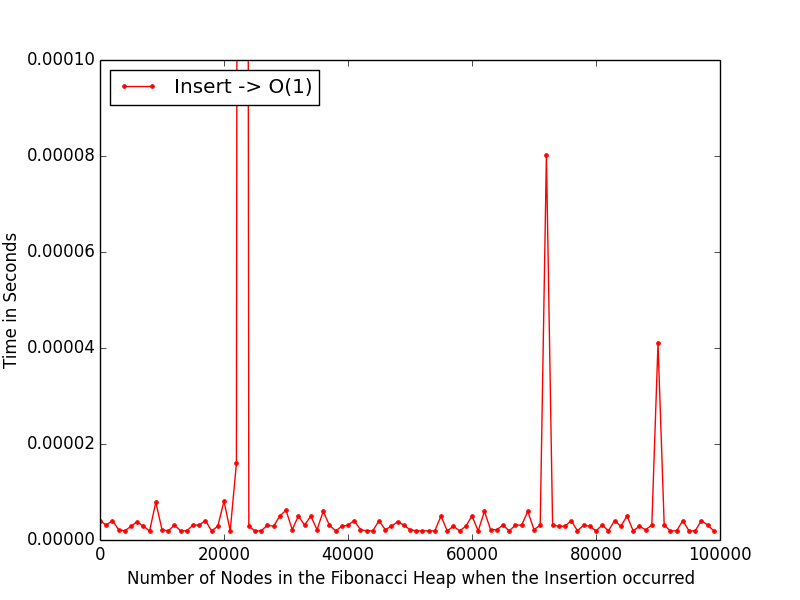
\includegraphics[width=0.95\columnwidth]{Figures/fibonacciHeapPerformanceInsert}
\caption{Insert Operation: $O(1)$}
\label{performanceInsert}
For Insertion operation, I created a new Fibonacci Heap with $n-1$ nodes and inserted the $n^{th}$ node. Since it is constant time operation, we can observe that irrespective of the number of nodes added, the time taken to add the $n^{th}$ node takes a constant time.
\end{figure}
\begin{figure}
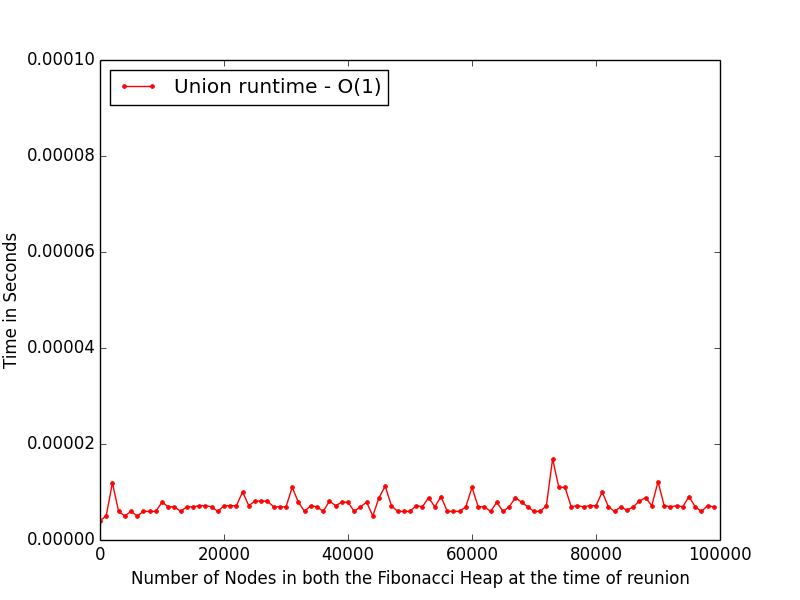
\includegraphics[width=0.95\columnwidth]{Figures/fibonacciHeapPerformanceUnion}
\caption{Union Operation: $O(1)$}
\label{performanceUnion}
For the Union operation, I created two Fibonacci Heap with $n$ nodes and then merged them. Since it is a constant time operation, we can observe that irrespective of the number of the nodes in both the Fibonacci Heap at the time of merging, the operation completes in a constant time.
\end{figure}
\begin{figure}
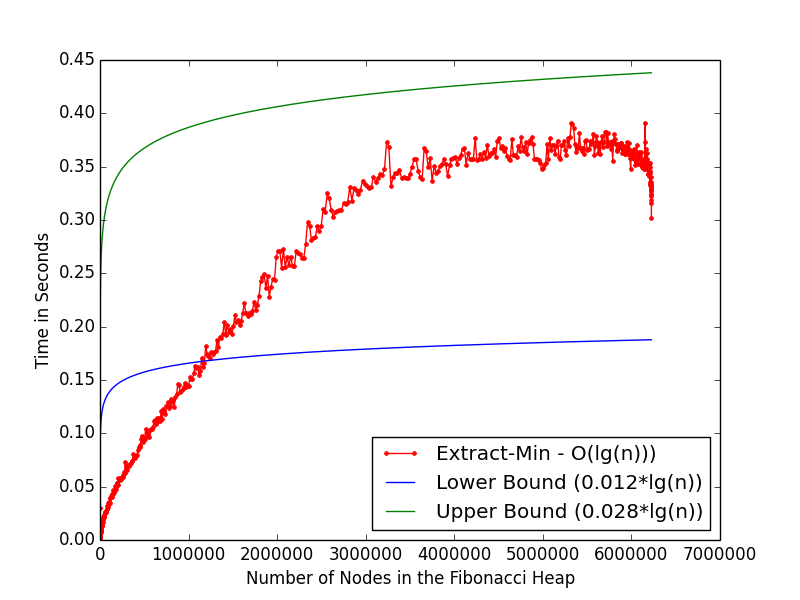
\includegraphics[width=0.95\columnwidth]{Figures/fibonacciHeapPerformanceExtractMin}
\caption{Extract Min Operation: $O(\log{n})^{*}$}
\label{performanceExtractMin}
For the Extract-Min operation, I create just one Fibonacci-Heap and keep adding nodes to it and perform Extract-Min operation at various stages. Since it has an amortized time bound , the extract-min operation at any stage is dependent on the previous stage when the extract-min operation occurred and hence I decided to use just one Fibonacci Heap for the entire analysis. I have a lower and upper bound with a constant time $\log{n}$ which shows that Extract-Min has an amortized time bound of $O(\log{n})$.\\ \textbf{Note: The X-axis is in log scale.}
\end{figure}
\begin{figure}
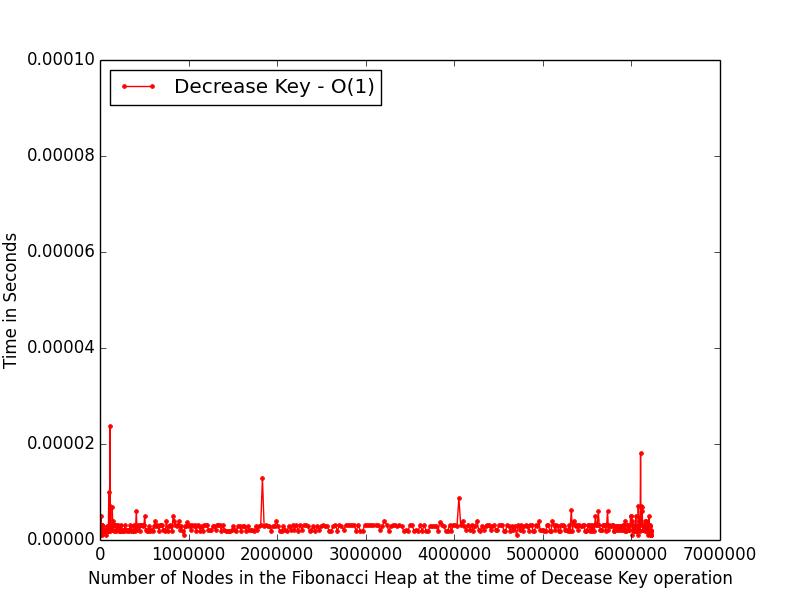
\includegraphics[width=0.95\columnwidth]{Figures/fibonacciHeapPerformanceDecreaseKey}
\caption{Decrease Key Operation: $O(1)^{*}$}
\label{performanceDecreaseKey}
For the Decrease-Key operation, I create a Fibonacci-Heap and add nodes to it. At various stages, I perform the decrease-key operation. I use a single Fibonacci-Heap since decrease-key runtime bound is amortized. The current decrease key operation runtime is based on when the previous decrease key operation was performed.\\ \textbf{Note: The X-axis is in log scale.}
\end{figure}
\begin{figure}
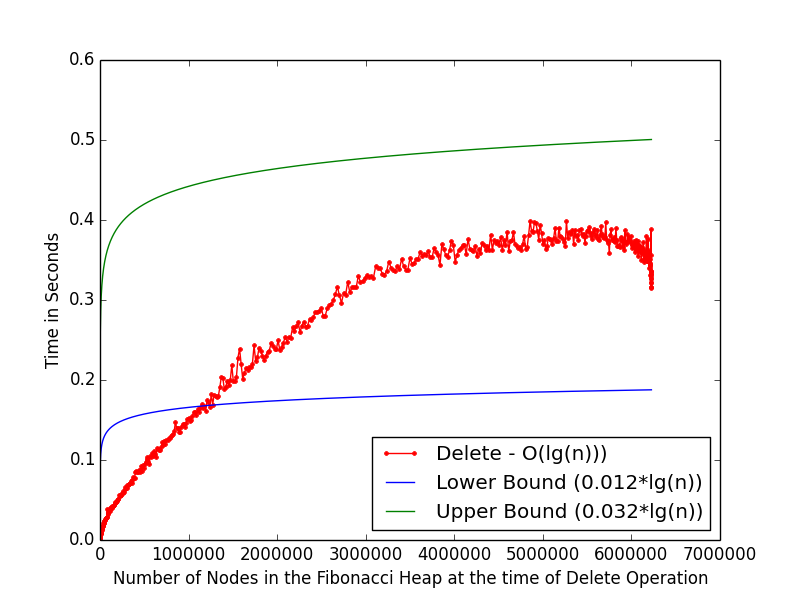
\includegraphics[width=0.95\columnwidth]{Figures/fibonacciHeapPerformanceDelete}
\caption{Delete Operation: $O(\log{n})^{*}$}
\label{performanceDelete}
For the Delete operation, I create just one Fibonacci-Heap and keep adding nodes to it and perform delete operation at various stages. Since it has an amortized time bound, the delete operation at any stage is dependent on the previous stage when the delete operation occurred and hence I decided to use just one Fibonacci Heap for the entire analysis. I have a lower and upper bound with a constant time $\log{n}$ which shows that Delete operation has an amortized time bound of $O(\log{n})$.\\ \textbf{Note: The X-axis is in log scale.}
\end{figure}


\section{Applications}
Generally in Network Optimization, the number of deletion operations is relatively small. Thus, Fibonacci Heaps can be used to obtain asymptotically faster algorithms. It is used in the following implementations ~\cite{fredman1987fibonacci} (Let $n$ be the number of vertices and $m$ be the number of edges):
\begin{itemize}
	\item Dijkstra's algorithm for the single-source shortest path program with non-negative edges. It improves the time bound to $O(n \log{n} + m)$  from previously best known time bound $O(m\log_{\frac{m}{n+2}}n)$
	\item All-pairs shortest path problem had a improvement of time bound to $O(n^2\log{n} + nm)$ from \\ $O(nm\log_{\frac{m}{n+2}}n)$
	\item Weight bipartite matching had improvement of time to $O(n^2\log{n} + nm)$ from $O(nm\log_{\frac{m}{n+2}}n$
	\item Minimum spanning tree problem had an improvement to $O(m\beta(m,n))$ from $O(m\log{\log_{\frac{m}{n+2}}n})$, where $\beta(m,n) = min\{i|\log^{(i)}n\} \leq \frac{m}{n}$. Note that $\beta(m,n) \leq \log^{*}n \ if \ m \geq n $
\end{itemize}


\bibliographystyle{abbrv}
\bibliography{fibonacciHeap}

%----------------------------------------------------------------------------------------


\end{document}